\documentclass[11pt,a4paper]{article}

% Image mode: pdf.
% Image paths stay relative. In PDF mode, place same-basename PDF conversions
% of the chapter SVG files in the assets/ directory beside this source.

\usepackage{iftex}
\ifPDFTeX
  \PackageError{handout}{This template requires XeTeX or Tectonic}{Compile with xelatex or tectonic.}
\fi

\usepackage[a4paper,top=18mm,bottom=20mm,left=20mm,right=20mm,headsep=6mm]{geometry}
\usepackage{fontspec}
\usepackage{xeCJK}
\usepackage{amsmath}
\usepackage{unicode-math}

% Font settings are intentionally visible in the generated .tex file.
% These defaults target the macOS machine used for the released PDF.
% Change the family names when compiling on another system.
\setmainfont{Songti TC}
\setsansfont{Heiti TC}
\setmonofont{Menlo}
\setCJKmainfont{Songti TC}
\setCJKsansfont{Heiti TC}
\setCJKmonofont{Heiti TC}
\setmathfont{STIX Two Math}
\XeTeXlinebreaklocale "zh"
\XeTeXlinebreakskip=0pt plus 1pt

\usepackage{xcolor}
\definecolor{HandoutBlue}{HTML}{215A91}
\definecolor{HandoutBlueLight}{HTML}{EEF5FC}
\definecolor{HandoutGreen}{HTML}{39715A}
\definecolor{HandoutGreenLight}{HTML}{EFF8F3}
\definecolor{HandoutGold}{HTML}{8A641C}
\definecolor{HandoutGoldLight}{HTML}{FFF8E8}
\definecolor{HandoutInk}{HTML}{253142}
\definecolor{HandoutMuted}{HTML}{667085}

\usepackage{graphicx}
\makeatletter
% Pandoc 3 emits an accessibility `alt` key for raster/PDF images. Older
% graphicx releases do not know that key, so accept it without changing layout.
\@ifundefined{KV@Gin@alt}{\define@key{Gin}{alt}{}}{}
\newsavebox\pandoc@box
\newcommand*\pandocbounded[1]{%
  \sbox\pandoc@box{#1}%
  \Gscale@div\@tempa{\textheight}{\dimexpr\ht\pandoc@box+\dp\pandoc@box\relax}%
  \Gscale@div\@tempb{\linewidth}{\wd\pandoc@box}%
  \ifdim\@tempb\p@<\@tempa\p@\let\@tempa\@tempb\fi
  \ifdim\@tempa\p@<\p@\scalebox{\@tempa}{\usebox\pandoc@box}%
  \else\usebox{\pandoc@box}%
  \fi
}
\makeatother
\usepackage{float}
\floatplacement{figure}{H}
% Pandoc uses LTcaptype=none for uncaptioned longtables. The caption package
% expects that name to exist as a counter even though it is never displayed.
\newcounter{none}
\usepackage{caption}
\captionsetup[figure]{labelformat=empty,labelsep=none,font=small}

\usepackage{booktabs,longtable,array,calc}
\usepackage{etoolbox}
\makeatletter
\patchcmd\longtable{\par}{\if@noskipsec\mbox{}\fi\par}{}{}
\makeatother

\usepackage[most]{tcolorbox}
\tcbuselibrary{breakable,skins}
\newtcolorbox{HandoutLearningMap}{
  enhanced,breakable,colback=HandoutBlueLight,colframe=HandoutBlue,
  boxrule=0.8pt,arc=1.5mm,left=3mm,right=3mm,top=2mm,bottom=2mm,
  before skip=8pt,after skip=10pt
}
\newtcolorbox{HandoutWorkedExample}{
  enhanced,breakable,colback=HandoutGreenLight,colframe=HandoutGreen,
  boxrule=0.65pt,arc=1.5mm,left=3mm,right=3mm,top=2mm,bottom=2mm,
  before skip=8pt,after skip=10pt
}
\newtcolorbox{HandoutSelfCheck}{
  enhanced,breakable,colback=HandoutGoldLight,colframe=HandoutGold,
  boxrule=0.65pt,arc=1.5mm,left=3mm,right=3mm,top=2mm,bottom=2mm,
  before skip=8pt,after skip=10pt
}

\usepackage{titlesec}
\titleformat{\section}{\sffamily\bfseries\Large\color{HandoutBlue}}{}{0pt}{}
\titleformat{\subsection}{\sffamily\bfseries\large\color{HandoutInk}}{}{0pt}{}
\titleformat{\subsubsection}{\sffamily\bfseries\normalsize\color{HandoutInk}}{}{0pt}{}
\titlespacing*{\section}{0pt}{1.4em}{0.55em}
\titlespacing*{\subsection}{0pt}{1.15em}{0.45em}
\titlespacing*{\subsubsection}{0pt}{0.9em}{0.35em}
\setcounter{secnumdepth}{-\maxdimen}

\usepackage{hyperref}
\usepackage{bookmark}
\IfFileExists{xurl.sty}{\usepackage{xurl}}{}
\urlstyle{same}
\hypersetup{
  colorlinks=true,
  linkcolor=HandoutBlue,
  urlcolor=HandoutBlue,
  citecolor=HandoutBlue,
  pdftitle={數A3-1 三角函數},
  pdfsubject={數學},
  pdfcreator={Pandoc with the HighSchooContent LaTeX template}
}

\setlength{\parindent}{0pt}
\setlength{\parskip}{0.55em plus 0.15em minus 0.1em}
\setlength{\emergencystretch}{3em}
\setlength{\LTpre}{0.5em}
\setlength{\LTpost}{0.5em}
\renewcommand{\arraystretch}{1.18}
\providecommand{\tightlist}{%
  \setlength{\itemsep}{0pt}\setlength{\parskip}{0pt}}
\pagestyle{plain}


\begin{document}

\begin{tcolorbox}[
  enhanced,colback=white,colframe=HandoutBlue,boxrule=1.1pt,arc=2mm,
  borderline west={3pt}{0pt}{HandoutBlue},left=5mm,right=4mm,top=4mm,bottom=4mm
]
{\sffamily\small\bfseries\color{HandoutBlue}學生講義}\par
{\sffamily\bfseries\LARGE\color{HandoutInk}數A3-1 三角函數}\par
\vspace{0.35em}{\large 用週期函數描述轉動，再合成同頻分量}\par
\vspace{0.45em}{\small\color{HandoutMuted}%
科目：數學
\quad 課程：普通高中數學A 第三冊
\quad 版本：學生版｜核心＋理解
\quad 校訂：2026-08-24
}\par
\vspace{0.25em}{\small\color{HandoutMuted}範圍：現行數學A主線}\par
\end{tcolorbox}


\begin{HandoutLearningMap}

\subsection{本章核心問題}\label{ux672cux7ae0ux6838ux5fc3ux554fux984c}

\begin{enumerate}
\def\labelenumi{\arabic{enumi}.}
\tightlist
\item
  \textbf{怎麼用圓本身來量角？}──弧度把角直接連到弧長與扇形面積。
\item
  \textbf{圓上的轉動怎麼變成波形？}──單位圓上的橫、縱坐標，攤開後就是 \(\cos\)、\(\sin\) 圖形。
\item
  \textbf{角相加時，函數值如何跟著改變？}──和差角是源頭，倍角與半角都可由它推導。
\item
  \textbf{為什麼 \(a\sin x+b\cos x\) 能合成一個波？}──同頻率是前提，振幅來自畢氏定理。
\end{enumerate}

弧度 → 三角函數圖形 → 圖形變換 → 和差角 → 倍角／半角 → 正餘弦疊合

{藍色：現行核心}
{青綠：理解支援}
{紫色：跨冊或高階延伸}

111--115 官方題本固定窗口中，5/5 份學測數學 A、3/5 份分科數學甲至少有一題把本章概念放在主幹或必要整合；這只描述已觀察試卷，不代表未來每年必考。

\end{HandoutLearningMap}

\section{三角函數如何描述轉動與週期訊號}\label{ux4e09ux89d2ux51fdux6578ux5982ux4f55ux63cfux8ff0ux8f49ux52d5ux8207ux9031ux671fux8a0aux865f}

\subsection{從轉角、分量到同頻訊號}\label{ux5f9eux8f49ux89d2ux5206ux91cfux5230ux540cux983bux8a0aux865f}

\textbf{弧度連結轉角、弧長與時間。} 圓周上的位移與角度可直接寫成 \(s=r\theta\)；採用弧度後，轉角、弧長與時間能放在同一個模型裡。

\textbf{圓周運動的坐標形成 sine 與 cosine。} 圓上轉動點的水平、鉛直坐標就是 \(r\cos\theta\)、\(r\sin\theta\)。旋轉零件的位置、週期感測訊號與規律振動，都可先用這兩個投影描述。

\textbf{和差角更新旋轉後的分量。} 裝置先朝角 \(A\)，再轉 \(B\)，新方向是 \(A+B\)；和差角公式把新方向分量改寫成舊方向與轉角的資料，適合更新導航或旋轉坐標。

\textbf{同頻分量可合成單一波。} 同頻的兩個 sine／cosine 分量相加後，仍是同一頻率，只改變振幅與相位。這能判斷同頻振動或訊號合成後會增強、減弱或延遲多少。

每個模型都有前提：輪子模型假設無滑動；週期模型適用於近似規律的區段；單一波疊合要求兩項同頻。這些前提界定公式可描述的現象與範圍。

\section{0. 從三角比延伸到三角函數}\label{ux5f9eux4e09ux89d2ux6bd4ux5ef6ux4f38ux5230ux4e09ux89d2ux51fdux6578}

在單位圓上，從正 \(x\) 軸逆時針轉過角 \(x\)，終邊與圓的交點記為 \(P\)。因半徑是 \(1\)，可寫成

\[
P=(\cos x,\sin x),
\qquad
\tan x=\frac{\sin x}{\cos x}\quad(\cos x\ne0).
\]

所以 \(\cos x\) 是點 \(P\) 的\textbf{橫坐標}，\(\sin x\) 是\textbf{縱坐標}；\(\tan x\) 是兩者的比。角 \(x\) 可取任意實數；\(\tan x\) 的定義域排除 \(\cos x=0\) 的角。三角比因此延伸為以角為輸入的三角函數。

點 \(P\) 位於半徑為 \(1\) 的圓上，因此其坐標滿足

\[
(\cos x)^2+(\sin x)^2=1.
\]

通常寫成

\[
\boxed{\sin^2x+\cos^2x=1}.
\]

這條關係直接來自單位圓方程 \(X^2+Y^2=1\)，後面的倍角公式與同角三角函數化簡都會使用它。

\subsection{廣義角、終邊與化簡}\label{ux5ee3ux7fa9ux89d2ux7d42ux908aux8207ux5316ux7c21}

角的始邊固定在正 \(x\) 軸；逆時針旋轉記為正角，順時針旋轉記為負角。旋轉任意圈數後停下的射線稱為\textbf{終邊}。兩角 \(\alpha,\beta\) 有相同終邊的條件是

\[
\boxed{\alpha=\beta+2k\pi},
\qquad k\in\mathbb Z.
\]

計算廣義角的三角函數時，先加減 \(2\pi\) 的整數倍，把角化到 \(0\le\theta<2\pi\)，再由終邊所在象限判斷正負：

{\def\LTcaptype{none} % do not increment counter
\begin{longtable}[]{@{}lrrr@{}}
\toprule\noalign{}
象限 & \(\sin\theta\) & \(\cos\theta\) & \(\tan\theta\) \\
\midrule\noalign{}
\endhead
\bottomrule\noalign{}
\endlastfoot
第一象限 & \(+\) & \(+\) & \(+\) \\
第二象限 & \(+\) & \(-\) & \(-\) \\
第三象限 & \(-\) & \(-\) & \(+\) \\
第四象限 & \(-\) & \(+\) & \(-\) \\
\end{longtable}
}

下列關係來自單位圓上的對稱與四分之一圈旋轉；各式在相應函數有定義時使用：

{\def\LTcaptype{none} % do not increment counter
\begin{longtable}[]{@{}
  >{\raggedright\arraybackslash}p{(\linewidth - 6\tabcolsep) * \real{0.2500}}
  >{\raggedright\arraybackslash}p{(\linewidth - 6\tabcolsep) * \real{0.2500}}
  >{\raggedright\arraybackslash}p{(\linewidth - 6\tabcolsep) * \real{0.2500}}
  >{\raggedright\arraybackslash}p{(\linewidth - 6\tabcolsep) * \real{0.2500}}@{}}
\toprule\noalign{}
\begin{minipage}[b]{\linewidth}\raggedright
角
\end{minipage} & \begin{minipage}[b]{\linewidth}\raggedright
sine
\end{minipage} & \begin{minipage}[b]{\linewidth}\raggedright
cosine
\end{minipage} & \begin{minipage}[b]{\linewidth}\raggedright
tangent
\end{minipage} \\
\midrule\noalign{}
\endhead
\bottomrule\noalign{}
\endlastfoot
\(-\theta\) & \(-\sin\theta\) & \(\cos\theta\) & \(-\tan\theta\) \\
\(\pi-\theta\) & \(\sin\theta\) & \(-\cos\theta\) & \(-\tan\theta\) \\
\(\pi+\theta\) & \(-\sin\theta\) & \(-\cos\theta\) & \(\tan\theta\) \\
\(\dfrac\pi2-\theta\) & \(\cos\theta\) & \(\sin\theta\) & \(\dfrac{\cos\theta}{\sin\theta}\) \\
\(\dfrac\pi2+\theta\) & \(\cos\theta\) & \(-\sin\theta\) & \(-\dfrac{\cos\theta}{\sin\theta}\) \\
\end{longtable}
}

例如 \(-7\pi/6\) 與 \(5\pi/6\) 相差 \(-2\pi\)，終邊同在第二象限，因此

\[
\sin\left(-\frac{7\pi}{6}\right)=\frac12,
\quad
\cos\left(-\frac{7\pi}{6}\right)=-\frac{\sqrt3}{2},
\quad
\tan\left(-\frac{7\pi}{6}\right)=-\frac{\sqrt3}{3}.
\]

下表並列常用角的度數、弧度與三角函數值。

{\def\LTcaptype{none} % do not increment counter
\begin{longtable}[]{@{}
  >{\raggedleft\arraybackslash}p{(\linewidth - 10\tabcolsep) * \real{0.1667}}
  >{\raggedleft\arraybackslash}p{(\linewidth - 10\tabcolsep) * \real{0.1667}}
  >{\raggedleft\arraybackslash}p{(\linewidth - 10\tabcolsep) * \real{0.1667}}
  >{\raggedleft\arraybackslash}p{(\linewidth - 10\tabcolsep) * \real{0.1667}}
  >{\raggedleft\arraybackslash}p{(\linewidth - 10\tabcolsep) * \real{0.1667}}
  >{\raggedleft\arraybackslash}p{(\linewidth - 10\tabcolsep) * \real{0.1667}}@{}}
\toprule\noalign{}
\begin{minipage}[b]{\linewidth}\raggedleft
角（度）
\end{minipage} & \begin{minipage}[b]{\linewidth}\raggedleft
\(0^\circ\)
\end{minipage} & \begin{minipage}[b]{\linewidth}\raggedleft
\(30^\circ\)
\end{minipage} & \begin{minipage}[b]{\linewidth}\raggedleft
\(45^\circ\)
\end{minipage} & \begin{minipage}[b]{\linewidth}\raggedleft
\(60^\circ\)
\end{minipage} & \begin{minipage}[b]{\linewidth}\raggedleft
\(90^\circ\)
\end{minipage} \\
\midrule\noalign{}
\endhead
\bottomrule\noalign{}
\endlastfoot
同一角（弧度） & \(0\) & \(\dfrac{\pi}{6}\) & \(\dfrac{\pi}{4}\) & \(\dfrac{\pi}{3}\) & \(\dfrac{\pi}{2}\) \\
\(\sin x\) & \(0\) & \(\dfrac12\) & \(\dfrac{\sqrt2}{2}\) & \(\dfrac{\sqrt3}{2}\) & \(1\) \\
\(\cos x\) & \(1\) & \(\dfrac{\sqrt3}{2}\) & \(\dfrac{\sqrt2}{2}\) & \(\dfrac12\) & \(0\) \\
\(\tan x\) & \(0\) & \(\dfrac{\sqrt3}{3}\) & \(1\) & \(\sqrt3\) & 未定義 \\
\end{longtable}
}

\subsection{函數圖形與圓周軌跡}\label{ux51fdux6578ux5716ux5f62ux8207ux5713ux5468ux8eccux8de1}

單位圓用來產生函數值；\(y=\sin x\) 的圖形則以「角 \(x\)」為橫軸、「函數值」為縱軸，記錄\textbf{輸入與輸出的關係}。圓周軌跡位於幾何平面，函數圖形位於輸入---輸出平面。

\section{1. 弧度：用弧長與半徑的比來量角}\label{ux5f27ux5ea6ux7528ux5f27ux9577ux8207ux534aux5f91ux7684ux6bd4ux4f86ux91cfux89d2}

\subsection{1.1 定義與換算}\label{ux5b9aux7fa9ux8207ux63dbux7b97}

在半徑為 \(r\) 的圓上，圓心角所對的弧長為 \(s\)。這個角的弧度定義為

\[
\boxed{\theta=\frac{s}{r}}
\]

同一個角畫在大小不同的圓上，\(s\) 與 \(r\) 會同比放大，因此 \(s/r\) 不變。弧度只取決於角度。

整圓的弧長是 \(2\pi r\)，所以一圈是 \(2\pi\) 弧度：

\[
360^\circ=2\pi\ \text{rad},
\qquad
180^\circ=\pi\ \text{rad}.
\]

因此

\[
\boxed{\text{度}\to\text{弧度：乘 }\frac{\pi}{180}},
\qquad
\boxed{\text{弧度}\to\text{度：乘 }\frac{180}{\pi}}.
\]

計算機必須使用與題目相同的角度模式：輸入 \(\sin30^\circ\) 時用 DEG（度），輸入 \(\sin(\pi/6)\) 時用 RAD（弧度）。兩者都應得到 \(1/2\)；答案不一致時，先檢查角度模式。

\begin{figure}
\centering
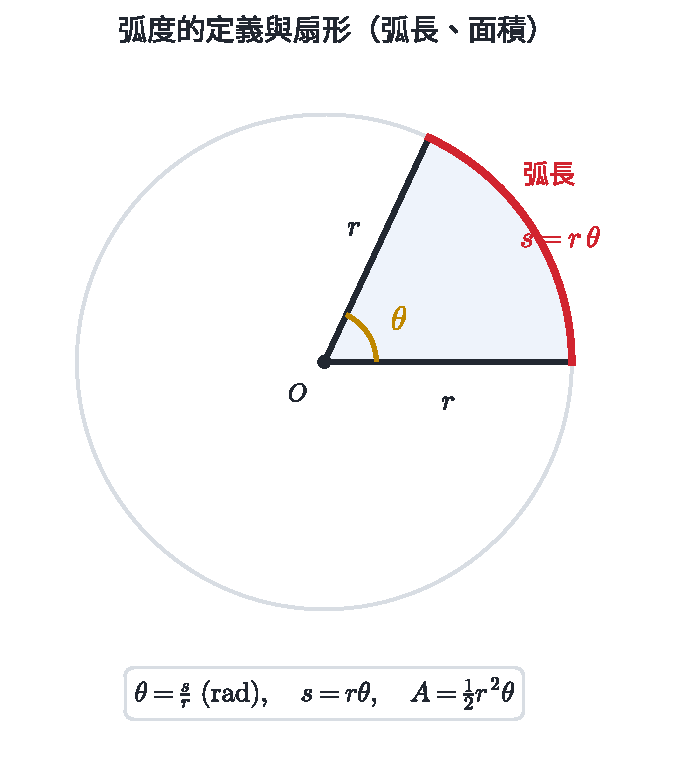
\includegraphics[width=0.88\linewidth,height=\textheight,keepaspectratio,alt={圖 1｜弧度是弧長與半徑的比；角固定時，圓放大不會改變這個比值。}]{assets/數A3-1-弧度扇形.pdf}
\caption{圖 1｜弧度是弧長與半徑的比；角固定時，圓放大不會改變這個比值。}
\end{figure}

\subsection{弧度如何直接連結角、弧長與位移？}\label{ux5f27ux5ea6ux5982ux4f55ux76f4ux63a5ux9023ux7d50ux89d2ux5f27ux9577ux8207ux4f4dux79fb}

弧度直接把定義 \(\theta=s/r\) 反解成 \(s=r\theta\)。角若用度數，弧長公式會多出 \(\pi/180\)；用弧度時，角與弧長共用同一個比例結構。

「rad」可保留來提醒角的量法；在公式運算中，\(s/r\) 的長度單位會相消。

\textbf{實務連結：旋轉編碼器與輪距。} 若編碼器量得輪子轉過 \(\theta\) 弧度，半徑為 \(r\)，理想無滑動時車輪前進距離就是 \(s=r\theta\)。若改用度數，程式每次都要再乘 \(\pi/180\)；弧度把感測角度直接接到幾何位移。輪胎打滑時，這個理想模型會高估或低估實際位移，需用其他感測資料校正。

\subsection{1.2 弧長與扇形面積}\label{ux5f27ux9577ux8207ux6247ux5f62ux9762ux7a4d}

由 \(\theta=s/r\) 直接得到弧長；扇形佔整圓的比例為 \(\theta/(2\pi)\)，因此

角 \(\theta\) \textbf{必須用弧度}時，

\[
\boxed{s=r\theta},
\qquad
\boxed{A=\frac12r^2\theta=\frac12rs}.
\]

\begin{HandoutWorkedExample}

\subsection{完整示範｜先換單位，再代公式}\label{ux5b8cux6574ux793aux7bc4ux5148ux63dbux55aeux4f4dux518dux4ee3ux516cux5f0f}

半徑 \(6\ \mathrm{cm}\) 的扇形，圓心角為 \(60^\circ\)。求弧長與面積。

\textbf{第一步：把角改成弧度}

\[
60^\circ=60\cdot\frac{\pi}{180}=\frac{\pi}{3}.
\]

\textbf{第二步：求弧長}

\[
s=r\theta=6\cdot\frac{\pi}{3}=2\pi\ \mathrm{cm}.
\]

\textbf{第三步：求面積}

\[
A=\frac12r^2\theta
=\frac12\cdot 6^2\cdot\frac{\pi}{3}
=6\pi\ \mathrm{cm^2}.
\]

\textbf{檢查}：\(60^\circ\) 是整圓的 \(1/6\)；弧長應為 \(12\pi/6=2\pi\)，面積應為 \(36\pi/6=6\pi\)，吻合。

\end{HandoutWorkedExample}

\subsection{\texorpdfstring{常見錯誤｜把 \(60\) 直接代入 \(s=r\theta\)}{常見錯誤｜把 60 直接代入 s=r\textbackslash theta}}\label{ux5e38ux898bux932fux8aa4ux628a-60-ux76f4ux63a5ux4ee3ux5165-srtheta}

\(s=r\theta\) 與 \(A=\tfrac12r^2\theta\) 已把角度換算吸收到定義裡，所以 \(\theta\) 必須是弧度。題目若給 \(60^\circ\)，應代 \(\pi/3\)；代入 \(60\) 會違反公式的弧度條件。

\begin{HandoutSelfCheck}

\subsection{練習｜弧度}\label{ux7df4ux7fd2ux5f27ux5ea6}

半徑 \(5\)、弧長 \(3\) 的圓弧所對圓心角是多少弧度？同一角若畫在半徑 \(10\) 的圓上，弧長是多少？

\textbf{答案：}\(\theta=s/r=3/5\)。角不變時，新弧長 \(s=r\theta=10\cdot(3/5)=6\)。

\end{HandoutSelfCheck}

\begin{HandoutWorkedExample}

\subsection{完整示範｜由扇形周長反求半徑}\label{ux5b8cux6574ux793aux7bc4ux7531ux6247ux5f62ux5468ux9577ux53cdux6c42ux534aux5f91}

一個圓心角為 \(2\) 弧度的扇形，周長為 \(20\ \mathrm{cm}\)。求半徑、弧長與面積。

扇形周長由兩條半徑與一段弧組成。設半徑為 \(r\)，則

\[
s=r\theta=2r,
\qquad
2r+s=20.
\]

代入 \(s=2r\)：

\[
4r=20,
\qquad
r=5\ \mathrm{cm}.
\]

所以

\[
s=2r=\boxed{10\ \mathrm{cm}},
\]

\[
A=\frac12rs
=\frac12\cdot5\cdot10
=\boxed{25\ \mathrm{cm^2}}.
\]

周長檢查：\(5+5+10=20\)，符合題目。

\end{HandoutWorkedExample}

\begin{HandoutSelfCheck}

\subsection{節末練習｜弧度、弧長與扇形}\label{ux7bc0ux672bux7df4ux7fd2ux5f27ux5ea6ux5f27ux9577ux8207ux6247ux5f62}

\begin{enumerate}
\def\labelenumi{\arabic{enumi}.}
\tightlist
\item
  把 \(135^\circ\) 化為弧度，把 \(-5\pi/6\) 化為度數。
\item
  半徑 \(12\ \mathrm{cm}\)、圓心角 \(5\pi/6\) 的扇形，求弧長與面積。
\item
  一個扇形的弧長為 \(10\)、面積為 \(30\)。求半徑與圓心角。
\item
  半徑 \(0.30\ \mathrm m\) 的輪子無滑動滾了 \(8\) 圈。輪心前進多少公尺？
\end{enumerate}

\textbf{答案：}

\begin{enumerate}
\def\labelenumi{\arabic{enumi}.}
\tightlist
\item
  \(135^\circ=3\pi/4\)；\(-5\pi/6=-150^\circ\)。
\item
  \(s=12(5\pi/6)=10\pi\ \mathrm{cm}\)；\(A=\tfrac12(12)^2(5\pi/6)=60\pi\ \mathrm{cm^2}\)。
\item
  由 \(A=\tfrac12rs\) 得 \(r=2A/s=6\)；\(\theta=s/r=5/3\) 弧度。
\item
  轉角為 \(16\pi\)，所以 \(s=r\theta=0.30(16\pi)=4.8\pi\ \mathrm m\)。
\end{enumerate}

\end{HandoutSelfCheck}

\section{2. 三角函數圖形：把單位圓攤開}\label{ux4e09ux89d2ux51fdux6578ux5716ux5f62ux628aux55aeux4f4dux5713ux6524ux958b}

\subsection{\texorpdfstring{2.1 \(\sin\)、\(\cos\)、\(\tan\) 的基本圖形}{2.1 \textbackslash sin、\textbackslash cos、\textbackslash tan 的基本圖形}}\label{sincostan-ux7684ux57faux672cux5716ux5f62}

讓點 \(P=(\cos x,\sin x)\) 沿單位圓逆時針轉動：

\begin{itemize}
\tightlist
\item
  \(\sin x\) 追蹤點的高度，所以從 \(0\) 上升到 \(1\)，再降到 \(-1\)，最後回到 \(0\)。
\item
  \(\cos x\) 追蹤水平位置，所以從 \(1\) 出發；它與 \(\sin x\) 形狀相同，但相位領先 \(\pi/2\)。
\item
  \(\tan x=\sin x/\cos x\)；當 \(\cos x=0\) 時沒有定義，因此圖形會出現鉛直漸近線。
\end{itemize}

\begin{figure}
\centering
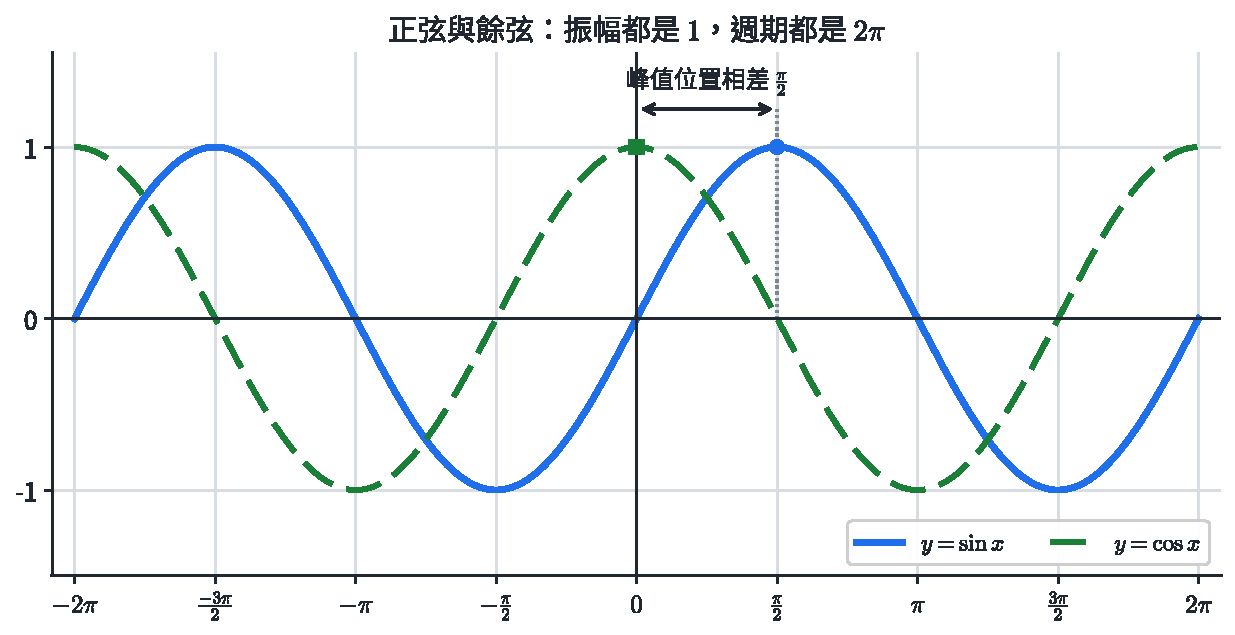
\includegraphics[width=0.96\linewidth,height=\textheight,keepaspectratio,alt={圖 2a｜cosine 的峰值在 x=0，sine 的峰值在 x=\textbackslash pi/2；兩者振幅、週期相同，峰值位置相差四分之一個週期。}]{assets/數A3-1-正弦餘弦圖.pdf}
\caption{圖 2a｜cosine 的峰值在 \(x=0\)，sine 的峰值在 \(x=\pi/2\)；兩者振幅、週期相同，峰值位置相差四分之一個週期。}
\end{figure}

\begin{figure}
\centering
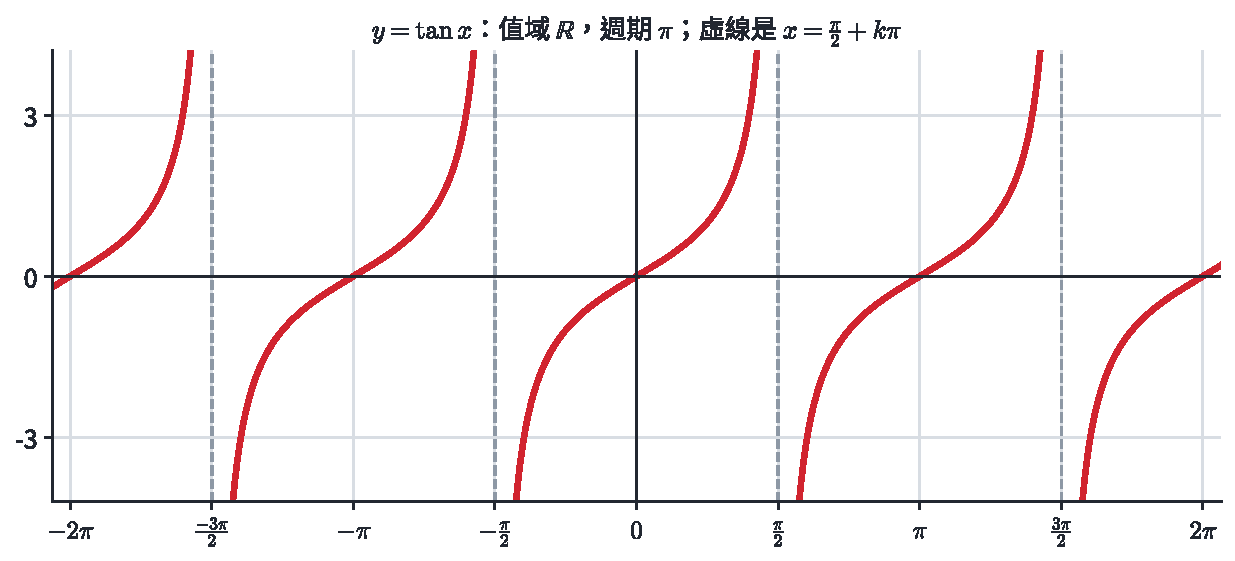
\includegraphics[width=0.96\linewidth,height=\textheight,keepaspectratio,alt={圖 2b｜tangent 的週期、零點與鉛直漸近線。}]{assets/數A3-1-正切函數圖.pdf}
\caption{圖 2b｜tangent 的週期、零點與鉛直漸近線。}
\end{figure}

圖 2a 的兩個峰值標記相隔 \(\pi/2\)，因此 \(\cos x\) 可視為 \(\sin x\) 向左平移 \(\pi/2\)。圖 2b 每兩條相鄰虛線之間是一個 tangent 分支；零點 \(k\pi\) 位於相鄰漸近線的中間。

{\def\LTcaptype{none} % do not increment counter
\begin{longtable}[]{@{}
  >{\raggedright\arraybackslash}p{(\linewidth - 10\tabcolsep) * \real{0.1579}}
  >{\raggedright\arraybackslash}p{(\linewidth - 10\tabcolsep) * \real{0.1579}}
  >{\raggedright\arraybackslash}p{(\linewidth - 10\tabcolsep) * \real{0.1579}}
  >{\raggedleft\arraybackslash}p{(\linewidth - 10\tabcolsep) * \real{0.2105}}
  >{\raggedright\arraybackslash}p{(\linewidth - 10\tabcolsep) * \real{0.1579}}
  >{\raggedright\arraybackslash}p{(\linewidth - 10\tabcolsep) * \real{0.1579}}@{}}
\toprule\noalign{}
\begin{minipage}[b]{\linewidth}\raggedright
函數
\end{minipage} & \begin{minipage}[b]{\linewidth}\raggedright
定義域
\end{minipage} & \begin{minipage}[b]{\linewidth}\raggedright
值域
\end{minipage} & \begin{minipage}[b]{\linewidth}\raggedleft
最小正週期
\end{minipage} & \begin{minipage}[b]{\linewidth}\raggedright
對稱性
\end{minipage} & \begin{minipage}[b]{\linewidth}\raggedright
零點
\end{minipage} \\
\midrule\noalign{}
\endhead
\bottomrule\noalign{}
\endlastfoot
\(y=\sin x\) & \(\mathbb R\) & \([-1,1]\) & \(2\pi\) & 奇函數 & \(x=k\pi\) \\
\(y=\cos x\) & \(\mathbb R\) & \([-1,1]\) & \(2\pi\) & 偶函數 & \(x=\dfrac\pi2+k\pi\) \\
\(y=\tan x\) & \(x\ne\dfrac\pi2+k\pi\) & \(\mathbb R\) & \(\pi\) & 奇函數 & \(x=k\pi\) \\
\end{longtable}
}

其中 \(k\in\mathbb Z\)。

\begin{HandoutSelfCheck}

\subsection{練習｜用基本圖形讀解}\label{ux7df4ux7fd2ux7528ux57faux672cux5716ux5f62ux8b80ux89e3}

在 \(0\le x<2\pi\) 中，\(\sin x=1/2\) 的解有哪些？\(\sin x>0\) 又對應哪一段區間？

\textbf{答案：}水平線 \(y=1/2\) 與 sine 圖交於 \(x=\pi/6,5\pi/6\)；圖形在 \(x\) 軸上方的區間是 \(0<x<\pi\)。

\end{HandoutSelfCheck}

\subsection{\texorpdfstring{為什麼 \(\cos\) 像 \(\sin\) 向左移 \(\pi/2\)？}{為什麼 \textbackslash cos 像 \textbackslash sin 向左移 \textbackslash pi/2？}}\label{ux70baux4ec0ux9ebc-cos-ux50cf-sin-ux5411ux5de6ux79fb-pi2}

點從 \((1,0)\) 出發時，橫坐標已是最大值 \(1\)，縱坐標則從 \(0\) 開始上升。因此 \(\cos\) 的相位比 \(\sin\) 領先四分之一圈：

\[
\boxed{\cos x=\sin\left(x+\frac\pi2\right)}.
\]

\textbf{實務連結：同一轉軸的兩個感測通道。} 若一個通道記錄圓上點的縱坐標，另一個記錄橫坐標，兩者形狀相同但相差四分之一圈。兩個通道在某一瞬間的讀值可幫助定位；連續追蹤轉動時，再看哪一個通道的變化領先，才可判斷轉動方向。這個判讀使用 \(\sin\)、\(\cos\) 的相位差。

\subsection{2.2 圖形變換：四個參數的作用}\label{ux5716ux5f62ux8b8aux63dbux56dbux500bux53c3ux6578ux7684ux4f5cux7528}

先排除常數函數的退化情形。對 \(A\ne0\)、\(B>0\)，把式子寫成

\[
y=A\sin\bigl(B(x-h)\bigr)+D
\]

或同型的 cosine 函數。四個參數的工作彼此分開：

{\def\LTcaptype{none} % do not increment counter
\begin{longtable}[]{@{}lll@{}}
\toprule\noalign{}
參數 & 幾何意義 & 可直接讀出的量 \\
\midrule\noalign{}
\endhead
\bottomrule\noalign{}
\endlastfoot
\(A\) & 鉛直伸縮；\(A<0\) 時再上下翻轉 & 振幅 \(|A|\) \\
\(B\) & 水平壓縮或拉伸 & 週期 \(T=2\pi/B\) \\
\(h\) & 水平平移 & 向右移 \(h\) \\
\(D\) & 鉛直平移 & 中線 \(y=D\)，值域 \([D-|A|,D+|A|]\) \\
\end{longtable}
}

若原式寫成 \(y=A\sin(Bx+C)+D\)，先提出 \(B\)：

\[
Bx+C=B\left(x+\frac{C}{B}\right)
=B\left(x-\left(-\frac CB\right)\right),
\]

所以相位移須由整理後的括號讀出，為 \(h=-C/B\)。

以下讀相位移時，一律保留題目所給 \(A\) 的正負號，再由 \(B(x-h)\) 讀取 \(h\)。相位表示並不唯一：\(h\) 可相差整數倍週期；若同時把 \(A\) 改號，還可得到相差半個週期的等價表示。

\begin{figure}
\centering
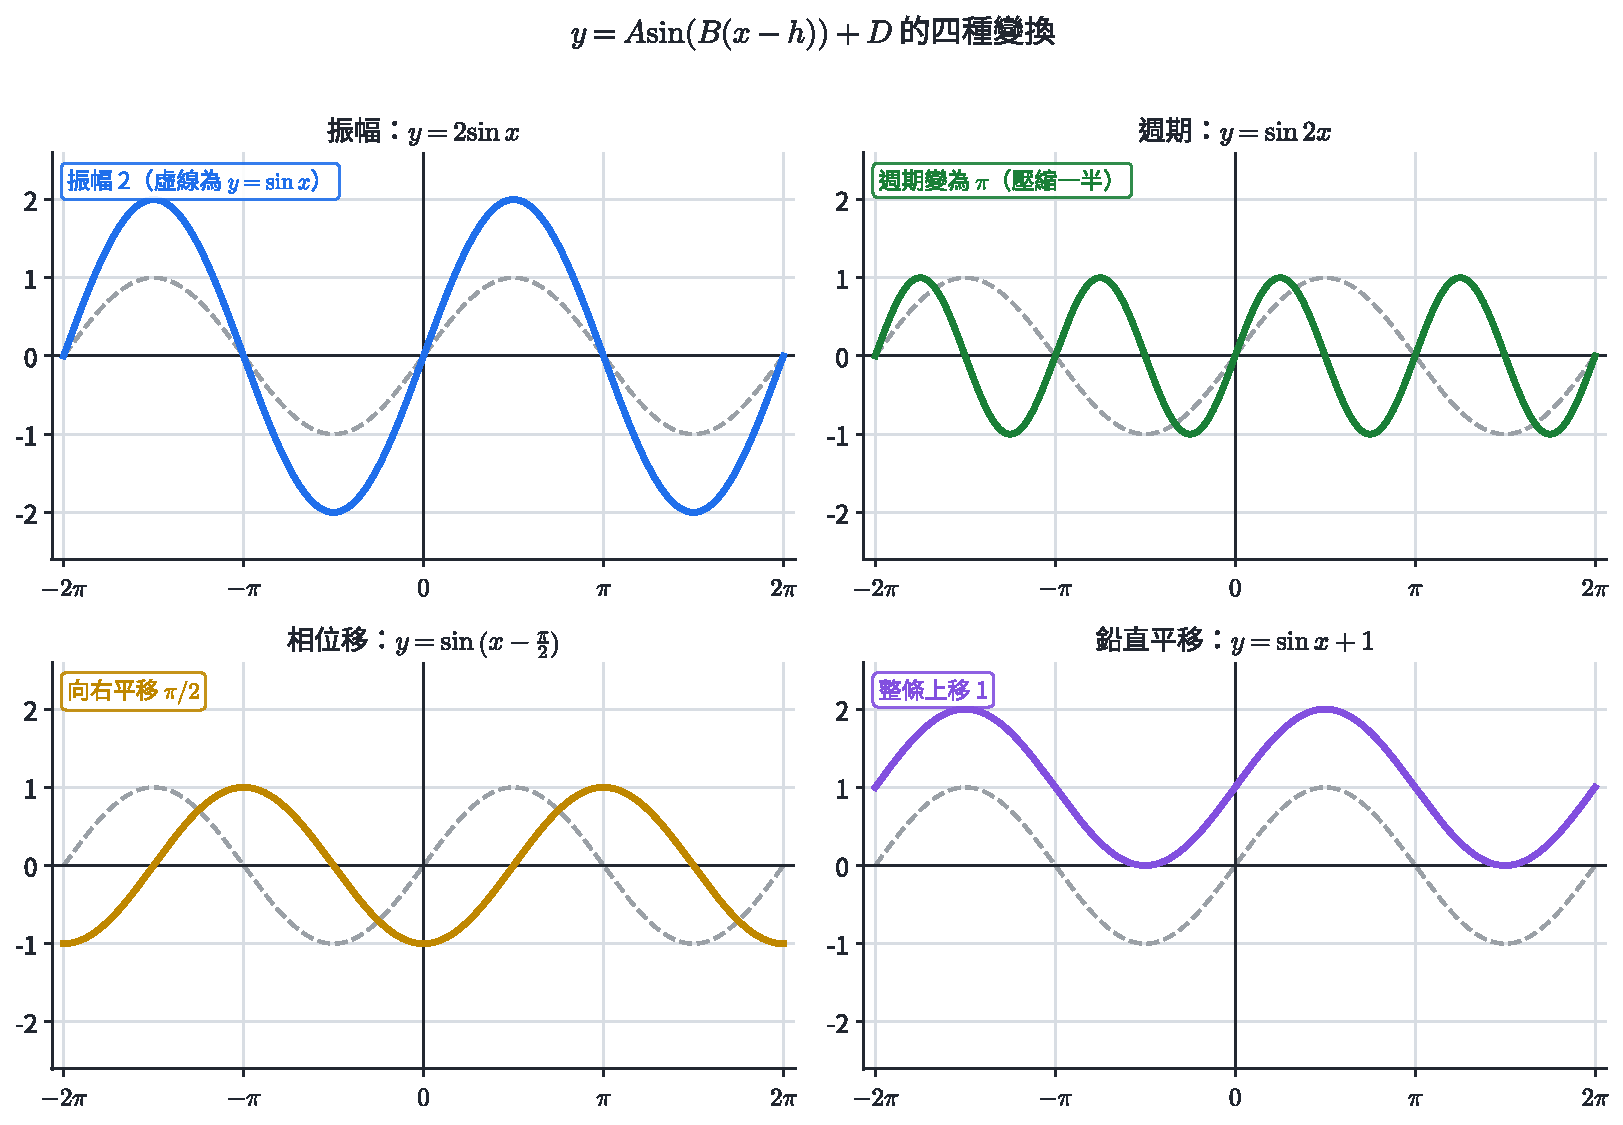
\includegraphics[width=0.96\linewidth,height=\textheight,keepaspectratio,alt={圖 3｜振幅、週期、水平平移與鉛直平移對圖形的作用。}]{assets/數A3-1-圖形變換.pdf}
\caption{圖 3｜振幅、週期、水平平移與鉛直平移對圖形的作用。}
\end{figure}

圖 3 四格都以灰色虛線 \(y=\sin x\) 為基準：比較波峰高度可讀振幅，比較相鄰波峰的水平距離可讀週期，比較對應波峰位置可讀相位移，比較中線高度可讀鉛直平移。

\begin{HandoutWorkedExample}

\subsection{完整示範｜讀出四個參數}\label{ux5b8cux6574ux793aux7bc4ux8b80ux51faux56dbux500bux53c3ux6578}

分析

\[
y=-3\cos\left(2x-\frac\pi3\right)+1.
\]

先整理括號：

\[
2x-\frac\pi3=2\left(x-\frac\pi6\right).
\]

因此：

\begin{itemize}
\tightlist
\item
  振幅 \(|-3|=3\)，負號表示上下翻轉。
\item
  週期 \(T=2\pi/2=\pi\)。
\item
  向右平移 \(\pi/6\)。
\item
  中線 \(y=1\)，值域 \([1-3,1+3]=[-2,4]\)。
\end{itemize}

\end{HandoutWorkedExample}

對同樣滿足 \(A\ne0\)、\(B>0\) 的 tangent 函數

\[
y=A\tan\bigl(B(x-h)\bigr)+D,
\]

週期是 \(\pi/B\)，中線是 \(y=D\)；它沒有振幅，因為值域沒有上下界。鉛直漸近線滿足

\[
B(x-h)=\frac\pi2+k\pi.
\]

\subsection{三個容易混淆的量}\label{ux4e09ux500bux5bb9ux6613ux6df7ux6dc6ux7684ux91cf}

\begin{itemize}
\tightlist
\item
  \textbf{振幅為 \(|A|\)}，其值非負。
\item
  \textbf{週期與 \(B\) 成反比}；\(B\) 越大，圖形在水平方向越密。
\item
  \textbf{tan 沒有振幅}；把它的垂直伸縮係數叫振幅，會把無界圖形誤當成上下有界。
\end{itemize}

\begin{HandoutSelfCheck}

\subsection{練習｜圖形與變換}\label{ux7df4ux7fd2ux5716ux5f62ux8207ux8b8aux63db}

\(y=2\sin\bigl(3(x+\pi/6)\bigr)-4\) 的振幅、週期、水平位移、中線與值域各為何？

\textbf{答案：}振幅 \(2\)；週期 \(2\pi/3\)；向左移 \(\pi/6\)；中線 \(y=-4\)；值域 \([-6,-2]\)。

\end{HandoutSelfCheck}

\subsection{2.3 由情境建立週期模型}\label{ux7531ux60c5ux5883ux5efaux7acbux9031ux671fux6a21ux578b}

若一個現象可近似為單一正弦或餘弦週期，可以用

\[
y=D+A\cos\bigl(B(x-h)\bigr)
\]

建立模型。固定依序回答四個問題：

\begin{enumerate}
\def\labelenumi{\arabic{enumi}.}
\tightlist
\item
  最高與最低值決定中線 \(D\) 與振幅 \(|A|\)。
\item
  週期 \(T\) 決定 \(B=2\pi/T\)。
\item
  一個已知的最高、最低或過中線位置決定 \(h\)。
\item
  把已知位置代回，確認函數值與變化方向。
\end{enumerate}

模型的寫法不唯一；使用 sine 或 cosine 都可以，重點是它符合題目的中線、振幅、週期與相位條件。真實現象通常只是\textbf{近似}週期模型，不必假裝完全正弦。

例如把旋轉標記在鉛直方向的位置記成 \(y(t)=D+A\sin(\omega t+\varphi)\)：\(D\) 是轉軸高度、\(|A|\) 是半徑、週期 \(T\) 給出 \(\omega=2\pi/T\)，\(\varphi\) 則記錄起始位置。四個參數各對應一個可量的物理量，這就是參數模型比「畫一條像波的曲線」更有用的地方。

\begin{HandoutWorkedExample}

\subsection{完整示範｜在指定區間解變形後的三角方程式}\label{ux5b8cux6574ux793aux7bc4ux5728ux6307ux5b9aux5340ux9593ux89e3ux8b8aux5f62ux5f8cux7684ux4e09ux89d2ux65b9ux7a0bux5f0f}

解

\[
2\sin\left(2x-\frac\pi6\right)=1,
\qquad 0\le x<2\pi.
\]

令 \(u=2x-\pi/6\)，則 \(\sin u=1/2\)。其一般解可分成兩族：

\[
u=\frac\pi6+2k\pi
\quad\text{或}\quad
u=\frac{5\pi}{6}+2k\pi,
\qquad k\in\mathbb Z.
\]

代回第一族：

\[
2x-\frac\pi6=\frac\pi6+2k\pi
\Longrightarrow
x=\frac\pi6+k\pi.
\]

代回第二族：

\[
2x-\frac\pi6=\frac{5\pi}{6}+2k\pi
\Longrightarrow
x=\frac\pi2+k\pi.
\]

篩選 \(0\le x<2\pi\)，得到

\[
\boxed{x=\frac\pi6,\ \frac\pi2,\ \frac{7\pi}{6},\ \frac{3\pi}{2}}.
\]

係數 \(2\) 使原區間內包含兩個完整 sine 週期，因此共有四個交點。

\end{HandoutWorkedExample}

\begin{HandoutWorkedExample}

\subsection{完整示範｜由起始狀態建立摩天輪高度模型}\label{ux5b8cux6574ux793aux7bc4ux7531ux8d77ux59cbux72c0ux614bux5efaux7acbux6469ux5929ux8f2aux9ad8ux5ea6ux6a21ux578b}

摩天輪半徑為 \(8\ \mathrm m\)，圓心離地 \(10\ \mathrm m\)，轉一圈需 \(40\ \mathrm s\)。座艙在 \(t=0\) 時位於最低點，且等速轉動。建立高度 \(h(t)\)，並求 \(t=10\) 時的高度。

中線為 \(10\)，振幅為 \(8\)，角頻率為

\[
B=\frac{2\pi}{T}=\frac{2\pi}{40}=\frac\pi{20}.
\]

\(t=0\) 在最低點，使用負 cosine 可直接符合初值：

\[
\boxed{h(t)=10-8\cos\left(\frac{\pi t}{20}\right)}.
\]

當 \(t=10\)：

\[
h(10)=10-8\cos\frac\pi2=\boxed{10\ \mathrm m}.
\]

此時經過四分之一週期，座艙應通過中線；計算結果與運動狀態一致。

\end{HandoutWorkedExample}

\begin{HandoutSelfCheck}

\subsection{節末練習｜圖形、方程式與週期模型}\label{ux7bc0ux672bux7df4ux7fd2ux5716ux5f62ux65b9ux7a0bux5f0fux8207ux9031ux671fux6a21ux578b}

\begin{enumerate}
\def\labelenumi{\arabic{enumi}.}
\tightlist
\item
  在 \(0\le x<2\pi\) 解 \(\tan x=\sqrt3\)。
\item
  在 \(0\le x\le2\pi\) 解不等式 \(\cos x\le-1/2\)。
\item
  \(y=-2\sin(\pi t/3)+5\) 的振幅、週期、中線與值域各為何？
\item
  求 \(y=2\tan\bigl(3(x-\pi/6)\bigr)\) 的最小正週期與所有鉛直漸近線。
\item
  某週期量最高為 \(14\)、最低為 \(6\)、週期為 \(8\)，且 \(t=1\) 時達最高值。用 cosine 建立一個模型。
\item
  在 \(0\le x<2\pi\) 解 \(\cos2x=0\)。
\end{enumerate}

\textbf{答案：}

\begin{enumerate}
\def\labelenumi{\arabic{enumi}.}
\tightlist
\item
  \(x=\pi/3,4\pi/3\)。
\item
  \(2\pi/3\le x\le4\pi/3\)。
\item
  振幅 \(2\)；週期 \(6\)；中線 \(y=5\)；值域 \([3,7]\)。
\item
  週期 \(\pi/3\)；漸近線 \(x=\pi/3+k\pi/3\)，\(k\in\mathbb Z\)。
\item
  \(y=10+4\cos\bigl(\tfrac\pi4(t-1)\bigr)\)。
\item
  \(x=\pi/4,3\pi/4,5\pi/4,7\pi/4\)。
\end{enumerate}

\end{HandoutSelfCheck}

\section{3. 和差角、倍角與半角：一條公式鏈}\label{ux548cux5deeux89d2ux500dux89d2ux8207ux534aux89d2ux4e00ux689dux516cux5f0fux93c8}

\subsection{3.1 和差角公式}\label{ux548cux5deeux89d2ux516cux5f0f}

\(\sin(A+B)\) 一般不等於 \(\sin A+\sin B\)。角度相加後，新的橫、縱坐標要同時混合原來兩個角的資訊：

\[
\boxed{\sin(A\pm B)=\sin A\cos B\pm\cos A\sin B}
\]

\[
\boxed{\cos(A\pm B)=\cos A\cos B\mp\sin A\sin B}
\]

當各項有意義時，

\[
\boxed{\tan(A\pm B)=\frac{\tan A\pm\tan B}{1\mp\tan A\tan B}}.
\]

記號結構是：\(\sin\) 的內外符號相同；\(\cos\) 的內外符號相反。下列距離推導說明這組公式的共同來源。

\subsection{\texorpdfstring{\(\cos(A-B)\) 如何由同一段距離推導？}{\textbackslash cos(A-B) 如何由同一段距離推導？}}\label{cosa-b-ux5982ux4f55ux7531ux540cux4e00ux6bb5ux8dddux96e2ux63a8ux5c0e}

在單位圓取

\[
P=(\cos A,\sin A),\qquad Q=(\cos B,\sin B).
\]

用坐標距離公式計算 \(PQ^2\)，得到

\[
PQ^2=2-2(\cos A\cos B+\sin A\sin B).
\]

另一方面，令 \(\delta\in[0,\pi]\) 是射線 \(OP\)、\(OQ\) 的較小夾角。\(\delta\) 與 \(A-B\) 只差正負號或整圈，所以 \(\cos\delta=\cos(A-B)\)。三角形 \(POQ\) 的兩邊都是 \(1\)；用餘弦定理得到

\[
PQ^2=2-2\cos(A-B).
\]

兩式代表同一段距離，因此

\[
\boxed{\cos(A-B)=\cos A\cos B+\sin A\sin B}.
\]

把 \(B\) 換成 \(-B\)，配合奇偶性可得 cosine 和角式；再配合餘角關係可得 sine 和差角式。兩式相除便得到 tangent 公式（各分母有意義時）。

\textbf{實務連結：更新方向分量。} 朝向角 \(A\) 的單位方向為 \((\cos A,\sin A)\)；再轉 \(B\) 後變成 \((\cos(A+B),\sin(A+B))\)。導航、機械手臂與電腦圖學都用這組關係更新二維方向；矩陣表示留待後續課程。

\begin{figure}
\centering
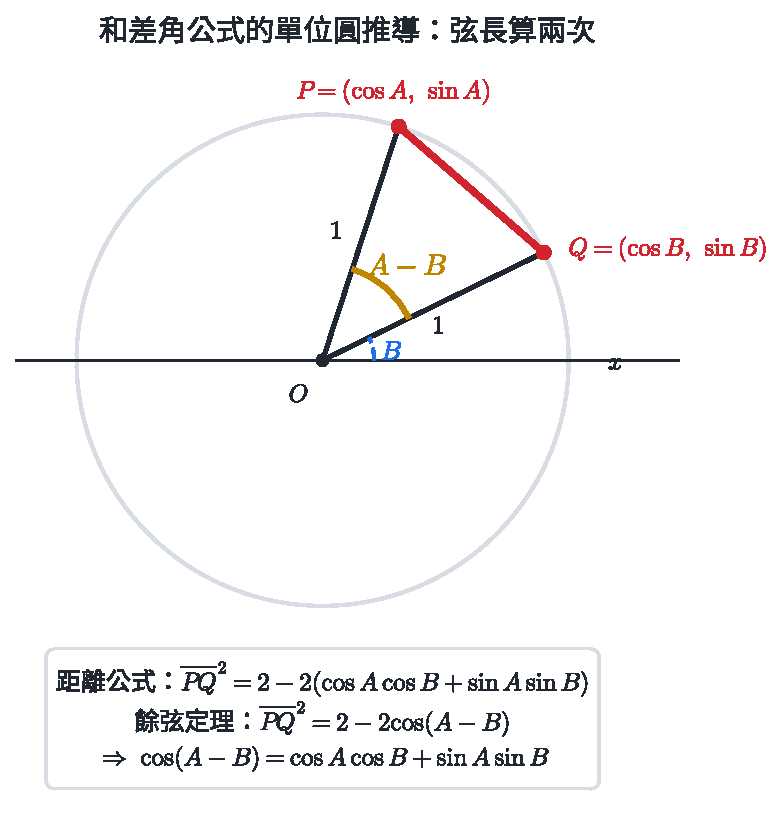
\includegraphics[width=0.84\linewidth,height=\textheight,keepaspectratio,alt={圖 4｜單位圓上兩點的距離，可用坐標距離公式與餘弦定理各算一次。}]{assets/數A3-1-和差角推導.pdf}
\caption{圖 4｜單位圓上兩點的距離，可用坐標距離公式與餘弦定理各算一次。}
\end{figure}

\begin{HandoutWorkedExample}

\subsection{\texorpdfstring{完整示範｜求 \(\sin75^\circ\) 的精確值}{完整示範｜求 \textbackslash sin75\^{}\textbackslash circ 的精確值}}\label{ux5b8cux6574ux793aux7bc4ux6c42-sin75circ-ux7684ux7cbeux78baux503c}

把 \(75^\circ\) 拆成兩個已知特殊角：

\[
\begin{aligned}
\sin75^\circ
&=\sin(45^\circ+30^\circ)\\
&=\sin45^\circ\cos30^\circ
 +\cos45^\circ\sin30^\circ\\
&=\frac{\sqrt2}{2}\cdot\frac{\sqrt3}{2}
 +\frac{\sqrt2}{2}\cdot\frac12\\
&=\boxed{\frac{\sqrt6+\sqrt2}{4}}.
\end{aligned}
\]

大小檢查：\(75^\circ\) 在第一象限且接近 \(90^\circ\)，答案應為接近 \(1\) 的正數；近似值約 \(0.966\)，合理。

\end{HandoutWorkedExample}

\subsection{3.2 倍角公式：令兩角相同}\label{ux500dux89d2ux516cux5f0fux4ee4ux5169ux89d2ux76f8ux540c}

在和角公式中令 \(B=A\)：

\[
\boxed{\sin2A=2\sin A\cos A}
\]

\[
\boxed{\cos2A=\cos^2A-\sin^2A
=1-2\sin^2A
=2\cos^2A-1}
\]

\[
\boxed{\tan2A=\frac{2\tan A}{1-\tan^2A}}
\]

最後一式只在分母與相關 tangent 值有意義時使用。

\(\cos2A\) 有三種寫法，選擇的原則是「想留下哪一種函數」：要只留 \(\sin A\)，用 \(1-2\sin^2A\)；要只留 \(\cos A\)，用 \(2\cos^2A-1\)。

\subsection{3.3 半角公式：把倍角反解}\label{ux534aux89d2ux516cux5f0fux628aux500dux89d2ux53cdux89e3}

把 \(\cos2A=1-2\sin^2A=2\cos^2A-1\) 反解，再令 \(2A=\theta\)：

\[
\boxed{\sin^2\frac\theta2=\frac{1-\cos\theta}{2}},
\qquad
\boxed{\cos^2\frac\theta2=\frac{1+\cos\theta}{2}}.
\]

需要 \(\sin(\theta/2)\) 或 \(\cos(\theta/2)\) 時，開根號後的正負號由 \(\theta/2\) 所在象限決定。

\subsection{常見錯誤｜半角公式開根號後一律取正}\label{ux5e38ux898bux932fux8aa4ux534aux89d2ux516cux5f0fux958bux6839ux865fux5f8cux4e00ux5f8bux53d6ux6b63}

平方只保留大小，會遺失正負號。例如 \(\theta/2\) 若在第二象限，\(\sin(\theta/2)>0\)、\(\cos(\theta/2)<0\)。正確流程是：\textbf{先算平方值，再判半角象限，最後決定符號。}

\begin{HandoutSelfCheck}

\subsection{練習｜公式鏈}\label{ux7df4ux7fd2ux516cux5f0fux93c8}

若 \(\sin\alpha=3/5\) 且 \(\alpha\) 在第二象限，求 \(\cos2\alpha\)。

\textbf{答案：}可直接用 \(\cos2\alpha=1-2\sin^2\alpha=1-2(9/25)=7/25\)。此題不必先求帶負號的 \(\cos\alpha\)。

\end{HandoutSelfCheck}

當 \(\sin\theta\) 與相應分母有意義時，半角的 tangent 還可寫成

\[
\boxed{
\tan\frac\theta2
=\frac{\sin\theta}{1+\cos\theta}
=\frac{1-\cos\theta}{\sin\theta}
}.
\]

第一式由 \(\sin\theta=2\sin(\theta/2)\cos(\theta/2)\) 與 \(1+\cos\theta=2\cos^2(\theta/2)\) 相除得到；第二式則使用 \(1-\cos\theta=2\sin^2(\theta/2)\)。這兩式保留半角的正負號，使用時仍須確認分母不為 \(0\)。

\begin{HandoutWorkedExample}

\subsection{完整示範｜用 tangent 和角公式求精確值}\label{ux5b8cux6574ux793aux7bc4ux7528-tangent-ux548cux89d2ux516cux5f0fux6c42ux7cbeux78baux503c}

\[
\begin{aligned}
\tan75^\circ
&=\tan(45^\circ+30^\circ)\\
&=\frac{1+1/\sqrt3}{1-1/\sqrt3}\\
&=\frac{\sqrt3+1}{\sqrt3-1}\\
&=\boxed{2+\sqrt3}.
\end{aligned}
\]

\(75^\circ\) 位於第一象限且接近 \(90^\circ\)，tangent 應為大於 \(1\) 的正數，符號與大小都合理。

\end{HandoutWorkedExample}

\begin{HandoutWorkedExample}

\subsection{完整示範｜半角值由整角與象限共同決定}\label{ux5b8cux6574ux793aux7bc4ux534aux89d2ux503cux7531ux6574ux89d2ux8207ux8c61ux9650ux5171ux540cux6c7aux5b9a}

已知 \(\cos\theta=-7/25\) 且 \(\pi/2<\theta<\pi\)。求 \(\sin(\theta/2)\)、\(\cos(\theta/2)\) 與 \(\tan(\theta/2)\)。

因 \(\pi/4<\theta/2<\pi/2\)，半角在第一象限，sine、cosine 都取正：

\[
\sin\frac\theta2
=\sqrt{\frac{1-\cos\theta}{2}}
=\sqrt{\frac{1+7/25}{2}}
=\boxed{\frac45},
\]

\[
\cos\frac\theta2
=\sqrt{\frac{1+\cos\theta}{2}}
=\sqrt{\frac{1-7/25}{2}}
=\boxed{\frac35}.
\]

所以

\[
\tan\frac\theta2=\frac{4/5}{3/5}=\boxed{\frac43}.
\]

\end{HandoutWorkedExample}

\begin{HandoutSelfCheck}

\subsection{節末練習｜和差角、倍角與半角}\label{ux7bc0ux672bux7df4ux7fd2ux548cux5deeux89d2ux500dux89d2ux8207ux534aux89d2}

\begin{enumerate}
\def\labelenumi{\arabic{enumi}.}
\tightlist
\item
  求 \(\cos15^\circ\) 的精確值。
\item
  求 \(\tan105^\circ\) 的精確值。
\item
  已知 \(\sin\alpha=-5/13\) 且 \(\alpha\) 在第四象限，求 \(\sin2\alpha\) 與 \(\cos2\alpha\)。
\item
  已知 \(\cos\theta=5/13\) 且 \(\pi<\theta<2\pi\)，求 \(\sin(\theta/2)\) 與 \(\cos(\theta/2)\)。
\item
  說明在兩邊都有定義時，為何 \((1-\cos2x)/\sin2x=\tan x\)。
\end{enumerate}

\textbf{答案：}

\begin{enumerate}
\def\labelenumi{\arabic{enumi}.}
\tightlist
\item
  \(\cos15^\circ=(\sqrt6+\sqrt2)/4\)。
\item
  \(\tan105^\circ=-(2+\sqrt3)\)。
\item
  \(\cos\alpha=12/13\)，所以 \(\sin2\alpha=-120/169\)、\(\cos2\alpha=119/169\)。
\item
  \(\theta/2\) 在第二象限，所以 \(\sin(\theta/2)=2\sqrt{13}/13\)、\(\cos(\theta/2)=-3\sqrt{13}/13\)。
\item
  \(1-\cos2x=2\sin^2x\)、\(\sin2x=2\sin x\cos x\)；約分後為 \(\tan x\)。原式要求 \(\sin2x\ne0\)，約分過程也在此條件下成立。
\end{enumerate}

\end{HandoutSelfCheck}

\section{4. 正餘弦疊合：兩個同頻分量合成一個波}\label{ux6b63ux9918ux5f26ux758aux5408ux5169ux500bux540cux983bux5206ux91cfux5408ux6210ux4e00ux500bux6ce2}

\subsection{4.1 公式與前提}\label{ux516cux5f0fux8207ux524dux63d0}

對不全為零的實數 \(p,q\)，可以把

\[
p\sin x+q\cos x
\]

寫成一個同頻率的正弦函數：

\[
\boxed{p\sin x+q\cos x=R\sin(x+\varphi)}
\]

其中

\[
\boxed{R=\sqrt{p^2+q^2}>0},
\qquad
\boxed{\cos\varphi=\frac pR,\quad \sin\varphi=\frac qR}.
\]

同一推導對任意 \(B>0\) 都成立：

\[
\boxed{p\sin(Bx)+q\cos(Bx)=R\sin(Bx+\varphi)}.
\]

因此合成後仍保留共同的週期 \(2\pi/B\)，也就是頻率不變；改變的是振幅與相位。

展開右式即可推導：

\[
R\sin(x+\varphi)
=(R\cos\varphi)\sin x+(R\sin\varphi)\cos x.
\]

比對係數，得到 \(R\cos\varphi=p\)、\(R\sin\varphi=q\)；平方相加後，因 \(\cos^2\varphi+\sin^2\varphi=1\)，便有 \(R=\sqrt{p^2+q^2}\)。

\begin{figure}
\centering
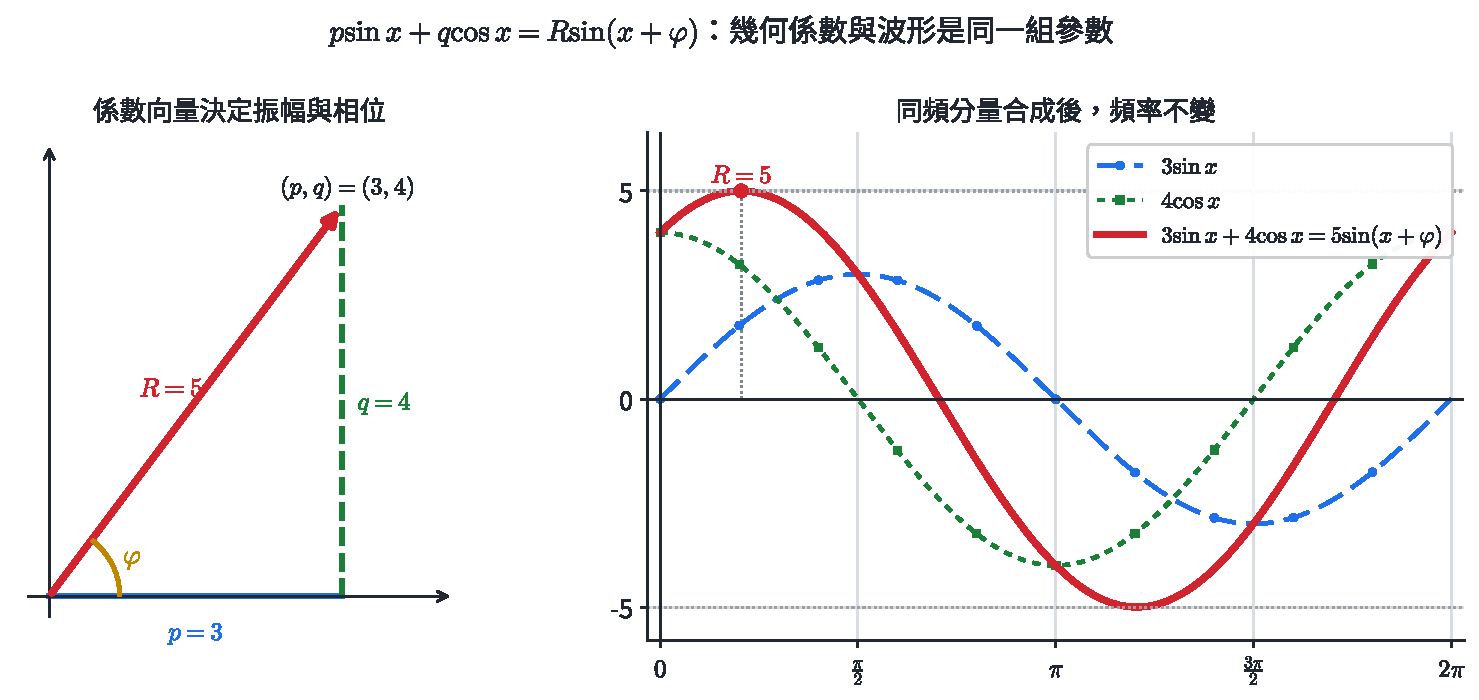
\includegraphics[width=0.96\linewidth,height=\textheight,keepaspectratio,alt={圖 5｜左圖用係數向量 (p,q) 讀出 R 與 \textbackslash varphi；右圖以同一組參數驗證兩個同頻分量合成單一正弦波。}]{assets/數A3-1-疊合.pdf}
\caption{圖 5｜左圖用係數向量 \((p,q)\) 讀出 \(R\) 與 \(\varphi\)；右圖以同一組參數驗證兩個同頻分量合成單一正弦波。}
\end{figure}

圖 5 左側的水平邊是 \(p=R\cos\varphi\)，鉛直邊是 \(q=R\sin\varphi\)，斜邊是 \(R\)；右側紅線的峰值 \(5\) 與左側斜邊 \(R=5\) 相同。

\subsection{\texorpdfstring{為什麼 \(R=\sqrt{p^2+q^2}\)？}{為什麼 R=\textbackslash sqrt\{p\^{}2+q\^{}2\}？}}\label{ux70baux4ec0ux9ebc-rsqrtp2q2}

條件 \(R\cos\varphi=p\)、\(R\sin\varphi=q\) 表示 \((p,q)\) 是一支長度為 \(R\)、方向角為 \(\varphi\) 的向量。因此 \(R\) 就是向量 \((p,q)\) 的長度，畢氏定理直接給出 \(R=\sqrt{p^2+q^2}\)。

決定 \(\varphi\) 時須同時看 \(p\)、\(q\) 的正負，以判斷 \((p,q)\) 所在象限；單用 \(\tan\varphi=q/p\) 會缺少相差 \(\pi\) 的象限資訊。

\textbf{實務連結：同頻訊號的增強與抵消。} 兩個相同頻率的量測通道相加時，可先各寫成 sine、cosine 分量，再以 \(R\) 與 \(\varphi\) 讀出合成振幅和延遲。若 \(R\) 變小，表示兩分量部分抵消；若變大，表示部分增強。不同頻率的訊號屬於多頻結構，需保留各自的頻率分量。

\subsection{適用範圍｜同頻分量的合成}\label{ux9069ux7528ux7bc4ux570dux540cux983bux5206ux91cfux7684ux5408ux6210}

\(p\sin x+q\cos x\) 的兩項共用同一個 \(x\)，所以能合成同頻波。\(\sin x+\cos2x\) 的頻率不同，應保留為兩個頻率分量。

\begin{HandoutWorkedExample}

\subsection{完整示範｜合成、求值域與最大位置}\label{ux5b8cux6574ux793aux7bc4ux5408ux6210ux6c42ux503cux57dfux8207ux6700ux5927ux4f4dux7f6e}

求

\[
f(x)=\sqrt3\sin x+\cos x
\]

的合成式、最大值，並找出 \(0\le x<2\pi\) 中取得最大值的位置。

由 \(p=\sqrt3,q=1\)：

\[
R=\sqrt{3+1}=2,
\qquad
\cos\varphi=\frac{\sqrt3}{2},
\quad
\sin\varphi=\frac12.
\]

所以 \(\varphi=\pi/6\)，

\[
f(x)=2\sin\left(x+\frac\pi6\right).
\]

最大值為 \(2\)。當

\[
x+\frac\pi6=\frac\pi2
\]

時取到，故 \(x=\pi/3\)。

\end{HandoutWorkedExample}

\begin{HandoutSelfCheck}

\subsection{練習｜疊合}\label{ux7df4ux7fd2ux758aux5408}

\(3\sin x-4\cos x\) 的最大值與最小值各是多少？不必先求相位。

\textbf{答案：}合成振幅 \(R=\sqrt{3^2+(-4)^2}=5\)，所以值域是 \([-5,5]\)；最大值 \(5\)，最小值 \(-5\)。

\end{HandoutSelfCheck}

\subsection{4.2 cosine 形式與限制區間極值}\label{cosine-ux5f62ux5f0fux8207ux9650ux5236ux5340ux9593ux6975ux503c}

同一個合成也可寫成 cosine 形式：

\[
\boxed{p\sin x+q\cos x=R\cos(x-\delta)},
\]

\[
R=\sqrt{p^2+q^2},
\qquad
\sin\delta=\frac pR,
\qquad
\cos\delta=\frac qR.
\]

正弦形式與餘弦形式描述同一條曲線；選擇哪一種，取決於題目給的是過中線位置還是最高、最低位置。求全體實數上的值域時，只需用 \(-1\le\sin u,\cos u\le1\)；求限制區間的極值時，還要把 \(u=x+\varphi\) 的實際範圍一起轉換。

\begin{HandoutWorkedExample}

\subsection{完整示範｜合成為 cosine 形式}\label{ux5b8cux6574ux793aux7bc4ux5408ux6210ux70ba-cosine-ux5f62ux5f0f}

令角 \(\alpha\) 滿足

\[
\sin\alpha=\frac35,
\qquad
\cos\alpha=\frac45,
\qquad 0<\alpha<\frac\pi2.
\]

則

\[
\begin{aligned}
-3\sin x+4\cos x
&=5\left(-\frac35\sin x+\frac45\cos x\right)\\
&=5(\cos x\cos\alpha-\sin x\sin\alpha)\\
&=\boxed{5\cos(x+\alpha)}.
\end{aligned}
\]

係數的平方和為 \(25\)，所以振幅為 \(5\)；展開結果也確實還原兩個係數。

\end{HandoutWorkedExample}

\begin{HandoutWorkedExample}

\subsection{完整示範｜限制區間內的最大值與最小值}\label{ux5b8cux6574ux793aux7bc4ux9650ux5236ux5340ux9593ux5167ux7684ux6700ux5927ux503cux8207ux6700ux5c0fux503c}

求

\[
f(x)=2\sin x+2\sqrt3\cos x,
\qquad 0\le x\le\frac\pi2
\]

的最大值、最小值及其位置。

先合成：

\[
f(x)=4\sin\left(x+\frac\pi3\right).
\]

當 \(0\le x\le\pi/2\) 時，

\[
\frac\pi3\le x+\frac\pi3\le\frac{5\pi}{6}.
\]

這段區間包含 \(\pi/2\)，所以最大值為

\[
\boxed{4},
\qquad x+\frac\pi3=\frac\pi2
\Longrightarrow x=\boxed{\frac\pi6}.
\]

最小值需比較兩個端點：

\[
f(0)=2\sqrt3,
\qquad
f\left(\frac\pi2\right)=2.
\]

故最小值為 \(\boxed{2}\)，在 \(x=\boxed{\pi/2}\) 取得。

\end{HandoutWorkedExample}

\subsection{4.3 合成後解方程式與不等式}\label{ux5408ux6210ux5f8cux89e3ux65b9ux7a0bux5f0fux8207ux4e0dux7b49ux5f0f}

合成把兩個同頻項化成單一三角函數，接著可用基本圖形處理交點與區間。例如

\[
\sqrt3\sin x+\cos x\ge1
\]

可化成

\[
2\sin\left(x+\frac\pi6\right)\ge1.
\]

在 \(0\le x<2\pi\) 中，\(x+\pi/6\) 的範圍是 \([\pi/6,13\pi/6)\)；配合 sine 圖形可得

\[
\boxed{0\le x\le\frac{2\pi}{3}}.
\]

\begin{HandoutSelfCheck}

\subsection{節末練習｜疊合、極值與解集}\label{ux7bc0ux672bux7df4ux7fd2ux758aux5408ux6975ux503cux8207ux89e3ux96c6}

\begin{enumerate}
\def\labelenumi{\arabic{enumi}.}
\tightlist
\item
  把 \(\sin x-\sqrt3\cos x\) 化為 \(R\sin(x+\varphi)\)，其中 \(-\pi<\varphi\le\pi\)。
\item
  求 \(5\sin x+12\cos x\) 在全體實數上的值域。
\item
  求 \(3\sin x+4\cos x\) 在 \(0\le x\le\pi/2\) 的最大值及位置。
\item
  在 \(0\le x<2\pi\) 解 \(\sin x-\cos x=0\)。
\item
  在 \(0\le x<2\pi\) 解 \(\sin x+\cos x>0\)。
\end{enumerate}

\textbf{答案：}

\begin{enumerate}
\def\labelenumi{\arabic{enumi}.}
\tightlist
\item
  \(2\sin(x-\pi/3)\)。
\item
  \([-13,13]\)。
\item
  最大值 \(5\)；令 \(0<\alpha<\pi/2\) 且 \(\sin\alpha=3/5\)、\(\cos\alpha=4/5\)，則在 \(x=\alpha\) 取得。
\item
  \(x=\pi/4,5\pi/4\)。
\item
  \(0\le x<3\pi/4\) 或 \(7\pi/4<x<2\pi\)。
\end{enumerate}

\end{HandoutSelfCheck}

\section{5. 一頁核心整理}\label{ux4e00ux9801ux6838ux5fc3ux6574ux7406}

\subsection{弧度}\label{ux5f27ux5ea6}

\begin{itemize}
\tightlist
\item
  \(\theta=s/r\)；\(180^\circ=\pi\) rad。
\item
  \(s=r\theta\)、\(A=\tfrac12r^2\theta=\tfrac12rs\)，其中 \(\theta\) 必須用弧度。
\end{itemize}

\subsection{圖形}\label{ux5716ux5f62}

\begin{itemize}
\tightlist
\item
  \(\sin\)、\(\cos\)：定義域 \(\mathbb R\)，值域 \([-1,1]\)，週期 \(2\pi\)。
\item
  \(\tan\)：\(x\ne\pi/2+k\pi\)，值域 \(\mathbb R\)，週期 \(\pi\)。
\item
  對 \(A\ne0\)、\(B\ne0\)，\(y=A\sin(B(x-h))+D\)：振幅 \(|A|\)、週期 \(2\pi/|B|\)、右移 \(h\)、中線 \(y=D\)。
\item
  在同一條件下，tangent 的週期為 \(\pi/|B|\)，沒有振幅。
\end{itemize}

\subsection{公式鏈}\label{ux516cux5f0fux93c8}

\begin{itemize}
\tightlist
\item
  和差角：\(\sin\) 同號、\(\cos\) 反號。
\item
  倍角：令兩角相同；\(\cos2A\) 有三種等價寫法。
\item
  半角：由倍角反解；開根號後要判 \(\theta/2\) 的象限。
\item
  \(\tan(\theta/2)=\sin\theta/(1+\cos\theta)=(1-\cos\theta)/\sin\theta\)，使用時保留分母條件。
\end{itemize}

\subsection{疊合}\label{ux758aux5408}

\begin{itemize}
\tightlist
\item
  \(p\sin(Bx)+q\cos(Bx)=R\sin(Bx+\varphi)\)；\(B\ne0\) 時，共同週期 \(2\pi/|B|\) 不變。
\item
  \(R=\sqrt{p^2+q^2}\)；\(\cos\varphi=p/R\)、\(\sin\varphi=q/R\)。
\item
  也可寫成 \(R\cos(Bx-\delta)\)；限制區間極值需同步轉換相位後的輸入範圍。
\item
  只適用同頻率的 sine、cosine 分量。
\end{itemize}

\section{6. 分層題與跨節整合題}\label{ux5206ux5c64ux984cux8207ux8de8ux7bc0ux6574ux5408ux984c}

\subsection{題目 1｜弧度、弧長與面積}\label{ux984cux76ee-1ux5f27ux5ea6ux5f27ux9577ux8207ux9762ux7a4d}

半徑 \(9\ \mathrm{cm}\) 的扇形，圓心角為 \(80^\circ\)。求其弧長與面積。

\subsection{題目 2｜依本章表示規範讀取圖形參數}\label{ux984cux76ee-2ux4f9dux672cux7ae0ux8868ux793aux898fux7bc4ux8b80ux53d6ux5716ux5f62ux53c3ux6578}

求

\[
y=-3\cos(2x-\pi)+1
\]

的振幅、週期、水平位移、中線與值域。

\subsection{題目 3｜tan 的週期與漸近線}\label{ux984cux76ee-3tan-ux7684ux9031ux671fux8207ux6f38ux8fd1ux7dda}

對 \(y=\tan2x\)，求最小正週期、所有零點與所有鉛直漸近線。

\subsection{題目 4｜建立週期模型}\label{ux984cux76ee-4ux5efaux7acbux9031ux671fux6a21ux578b}

某地一天的溫度可近似為正餘弦週期模型。最高溫 \(30^\circ\mathrm C\)、最低溫 \(18^\circ\mathrm C\)，週期 \(24\) 小時，且 \(t=6\) 時達最高溫。用 cosine 建立溫度 \(T(t)\)，並求 \(t=12\) 時的溫度。

\subsection{題目 5｜和角公式}\label{ux984cux76ee-5ux548cux89d2ux516cux5f0f}

不用計算機，求 \(\cos75^\circ\) 的精確值。

\subsection{題目 6｜半角與象限}\label{ux984cux76ee-6ux534aux89d2ux8207ux8c61ux9650}

已知 \(\cos\theta=-3/5\) 且 \(\pi/2<\theta<\pi\)，求

\[
\sin\frac\theta2,
\qquad
\cos\frac\theta2.
\]

\subsection{題目 7｜疊合與極值位置}\label{ux984cux76ee-7ux758aux5408ux8207ux6975ux503cux4f4dux7f6e}

將

\[
\sqrt3\sin x-\cos x
\]

化為 \(R\sin(x+\varphi)\)，並求 \(0\le x<2\pi\) 中取得最大值的 \(x\)。

\subsection{題目 8｜用疊合解方程式}\label{ux984cux76ee-8ux7528ux758aux5408ux89e3ux65b9ux7a0bux5f0f}

解

\[
\sin x+\cos x=1,
\qquad 0\le x<2\pi.
\]

\subsection{題目 9｜倍頻方程式}\label{ux984cux76ee-9ux500dux983bux65b9ux7a0bux5f0f}

解

\[
\cos2x=-\frac12,
\qquad 0\le x<2\pi.
\]

\subsection{題目 10｜tangent 差角}\label{ux984cux76ee-10tangent-ux5deeux89d2}

不用計算機，求 \(\tan15^\circ\) 的精確值。

\subsection{題目 11｜由 tangent 求倍角}\label{ux984cux76ee-11ux7531-tangent-ux6c42ux500dux89d2}

已知 \(\tan\alpha=2\) 且 \(\pi<\alpha<3\pi/2\)。求 \(\sin2\alpha\) 與 \(\cos2\alpha\)。

\subsection{題目 12｜cosine 型疊合}\label{ux984cux76ee-12cosine-ux578bux758aux5408}

令 \(0<\beta<\pi/2\) 且 \(\sin\beta=3/5\)、\(\cos\beta=4/5\)。把

\[
-3\sin x+4\cos x
\]

化為 \(R\cos(x+\beta)\)，並寫出值域。

\subsection{題目 13｜跨節整合：轉速、弧長與週期坐標}\label{ux984cux76ee-13ux8de8ux7bc0ux6574ux5408ux8f49ux901fux5f27ux9577ux8207ux9031ux671fux5750ux6a19}

半徑 \(0.40\ \mathrm m\) 的輪子以每分鐘 \(15\) 圈等速轉動，且無滑動。

\begin{enumerate}
\def\labelenumi{\arabic{enumi}.}
\tightlist
\item
  求角速度，單位用 \(\mathrm{rad/s}\)；
\item
  求 \(8\) 秒內輪心前進的距離；
\item
  輪緣標記在 \(t=0\) 位於輪心正上方。以輪心為原點、向上為正，寫出標記的鉛直坐標 \(y(t)\)。
\end{enumerate}

\subsection{題目 14｜跨節整合：圖形參數與不等式}\label{ux984cux76ee-14ux8de8ux7bc0ux6574ux5408ux5716ux5f62ux53c3ux6578ux8207ux4e0dux7b49ux5f0f}

對

\[
y=2\sin\left(2\left(x-\frac\pi4\right)\right)+1,
\]

\begin{enumerate}
\def\labelenumi{\arabic{enumi}.}
\tightlist
\item
  求振幅、週期、相位移、中線和值域；
\item
  在 \(0\le x<\pi\) 解 \(y\ge2\)。
\end{enumerate}

\subsection{題目 15｜跨節整合：先展開，再疊合}\label{ux984cux76ee-15ux8de8ux7bc0ux6574ux5408ux5148ux5c55ux958bux518dux758aux5408}

把

\[
\sin x+\sin\left(x+\frac\pi3\right)
\]

化為單一正弦函數，並求它在 \(0\le x<2\pi\) 的所有零點。

\subsection{題目 16｜跨節整合：由最高與最低時刻建模}\label{ux984cux76ee-16ux8de8ux7bc0ux6574ux5408ux7531ux6700ux9ad8ux8207ux6700ux4f4eux6642ux523bux5efaux6a21}

某港口潮位可近似為正餘弦模型。\(t=2\) 小時時潮位最高為 \(5.2\ \mathrm m\)，\(t=8\) 小時時潮位最低為 \(1.6\ \mathrm m\)，且這兩個時刻之間沒有其他最高或最低點。

\begin{enumerate}
\def\labelenumi{\arabic{enumi}.}
\tightlist
\item
  求中線、振幅與週期；
\item
  建立以 cosine 表示的潮位 \(H(t)\)；
\item
  求 \(t=5\) 時的潮位。
\end{enumerate}

\clearpage

\section{7. 分層題與跨節整合題詳解}\label{ux5206ux5c64ux984cux8207ux8de8ux7bc0ux6574ux5408ux984cux8a73ux89e3}

\subsection{第 1 題}\label{ux7b2c-1-ux984c}

先換成弧度：

\[
80^\circ=80\cdot\frac\pi{180}=\frac{4\pi}{9}.
\]

弧長：

\[
s=r\theta=9\cdot\frac{4\pi}{9}=\boxed{4\pi\ \mathrm{cm}}.
\]

面積：

\[
A=\frac12r^2\theta
=\frac12\cdot81\cdot\frac{4\pi}{9}
=\boxed{18\pi\ \mathrm{cm^2}}.
\]

\subsection{第 2 題}\label{ux7b2c-2-ux984c}

先整理括號：

\[
2x-\pi=2\left(x-\frac\pi2\right).
\]

依保留原式 \(A=-3\) 的表示規範，振幅為 \(3\)；週期為 \(2\pi/2=\pi\)；向右平移 \(\pi/2\)；中線為 \(y=1\)；值域為

\[
[1-3,1+3]=\boxed{[-2,4]}.
\]

外面的負號造成上下翻轉，但不改變振幅與值域端點。

相位表示並不唯一。等價地，

\[
-3\cos(2x-\pi)+1=3\cos2x+1,
\]

也可用「正振幅、不平移」表示；兩種寫法是同一個圖形。

\subsection{第 3 題}\label{ux7b2c-3-ux984c}

\(\tan u\) 的週期是 \(\pi\)。令 \(u=2x\)，輸入變快 2 倍，所以週期變成

\[
\boxed{\frac\pi2}.
\]

零點來自 \(2x=k\pi\)：

\[
\boxed{x=\frac{k\pi}{2}},\qquad k\in\mathbb Z.
\]

鉛直漸近線來自 \(2x=\pi/2+k\pi\)：

\[
\boxed{x=\frac\pi4+\frac{k\pi}{2}},\qquad k\in\mathbb Z.
\]

\subsection{第 4 題}\label{ux7b2c-4-ux984c}

中線與振幅分別是

\[
D=\frac{30+18}{2}=24,
\qquad
A=\frac{30-18}{2}=6.
\]

週期 \(24\)，所以角頻率係數

\[
B=\frac{2\pi}{24}=\frac\pi{12}.
\]

cosine 在輸入為 \(0\) 時取最大值，而最高溫發生於 \(t=6\)，可寫成

\[
\boxed{T(t)=24+6\cos\left(\frac\pi{12}(t-6)\right)}.
\]

代入 \(t=12\)：

\[
T(12)=24+6\cos\frac\pi2=\boxed{24^\circ\mathrm C}.
\]

\subsection{第 5 題}\label{ux7b2c-5-ux984c}

\[
\begin{aligned}
\cos75^\circ
&=\cos(45^\circ+30^\circ)\\
&=\cos45^\circ\cos30^\circ
-\sin45^\circ\sin30^\circ\\
&=\frac{\sqrt2}{2}\cdot\frac{\sqrt3}{2}
-\frac{\sqrt2}{2}\cdot\frac12\\
&=\boxed{\frac{\sqrt6-\sqrt2}{4}}.
\end{aligned}
\]

\subsection{第 6 題}\label{ux7b2c-6-ux984c}

由 \(\pi/2<\theta<\pi\) 可知 \(\pi/4<\theta/2<\pi/2\)，所以 \(\theta/2\) 在第一象限，sine、cosine 都取正。

\[
\sin^2\frac\theta2
=\frac{1-\cos\theta}{2}
=\frac{1+3/5}{2}
=\frac45,
\]

故

\[
\boxed{\sin\frac\theta2=\frac{2}{\sqrt5}=\frac{2\sqrt5}{5}}.
\]

同理

\[
\cos^2\frac\theta2
=\frac{1+\cos\theta}{2}
=\frac{1-3/5}{2}
=\frac15,
\]

所以

\[
\boxed{\cos\frac\theta2=\frac{1}{\sqrt5}=\frac{\sqrt5}{5}}.
\]

\subsection{第 7 題}\label{ux7b2c-7-ux984c}

令 \(p=\sqrt3,q=-1\)。則

\[
R=\sqrt{3+1}=2,
\qquad
\cos\varphi=\frac{\sqrt3}{2},
\quad
\sin\varphi=-\frac12.
\]

所以 \(\varphi=-\pi/6\)，

\[
\sqrt3\sin x-\cos x
=\boxed{2\sin\left(x-\frac\pi6\right)}.
\]

最大值為 \(2\)，當

\[
x-\frac\pi6=\frac\pi2
\]

時取得，因此在指定區間中

\[
\boxed{x=\frac{2\pi}{3}}.
\]

\subsection{第 8 題}\label{ux7b2c-8-ux984c}

先疊合：

\[
\sin x+\cos x
=\sqrt2\sin\left(x+\frac\pi4\right).
\]

因此

\[
\sin\left(x+\frac\pi4\right)=\frac{1}{\sqrt2}=\frac{\sqrt2}{2}.
\]

列出 sine 的一般解：

\[
x+\frac\pi4=\frac\pi4+2k\pi
\quad\text{或}\quad
x+\frac\pi4=\frac{3\pi}{4}+2k\pi,
\qquad k\in\mathbb Z.
\]

所以 \(x=2k\pi\) 或 \(x=\pi/2+2k\pi\)。篩選 \(0\le x<2\pi\)，得到

\[
\boxed{x=0\quad\text{或}\quad x=\frac\pi2}.
\]

兩值代回原式皆成立。

\subsection{第 9 題}\label{ux7b2c-9-ux984c}

令 \(u=2x\)。\(\cos u=-1/2\) 的一般解為

\[
u=\frac{2\pi}{3}+2k\pi
\quad\text{或}\quad
u=\frac{4\pi}{3}+2k\pi.
\]

除以 \(2\)：

\[
x=\frac\pi3+k\pi
\quad\text{或}\quad
x=\frac{2\pi}{3}+k\pi.
\]

篩選 \(0\le x<2\pi\)：

\[
\boxed{x=\frac\pi3,\ \frac{2\pi}{3},\ \frac{4\pi}{3},\ \frac{5\pi}{3}}.
\]

\subsection{第 10 題}\label{ux7b2c-10-ux984c}

把 \(15^\circ\) 寫成 \(45^\circ-30^\circ\)：

\[
\begin{aligned}
\tan15^\circ
&=\frac{\tan45^\circ-\tan30^\circ}
{1+\tan45^\circ\tan30^\circ}\\
&=\frac{1-1/\sqrt3}{1+1/\sqrt3}\\
&=\frac{\sqrt3-1}{\sqrt3+1}\\
&=\boxed{2-\sqrt3}.
\end{aligned}
\]

\(15^\circ\) 位於第一象限，結果約為 \(0.268\)，符號與大小合理。

\subsection{第 11 題}\label{ux7b2c-11-ux984c}

倍角可直接用 tangent 表示：

\[
\sin2\alpha=\frac{2\tan\alpha}{1+\tan^2\alpha},
\qquad
\cos2\alpha=\frac{1-\tan^2\alpha}{1+\tan^2\alpha}.
\]

代入 \(\tan\alpha=2\)：

\[
\boxed{\sin2\alpha=\frac45},
\qquad
\boxed{\cos2\alpha=-\frac35}.
\]

\(\alpha\) 在第三象限，所以 \(2\alpha\) 扣除一圈後落在第一或第二象限；由 \(\tan\alpha=2>1\) 可知 \(2\alpha\) 的 cosine 為負，與結果一致。

\subsection{第 12 題}\label{ux7b2c-12-ux984c}

由題設的 \(\beta\)：

\[
\begin{aligned}
5\cos(x+\beta)
&=5(\cos x\cos\beta-\sin x\sin\beta)\\
&=5\left(\frac45\cos x-\frac35\sin x\right)\\
&=-3\sin x+4\cos x.
\end{aligned}
\]

因此

\[
\boxed{-3\sin x+4\cos x=5\cos(x+\beta)}.
\]

因 \(-1\le\cos(x+\beta)\le1\)，值域為 \(\boxed{[-5,5]}\)。

\subsection{第 13 題}\label{ux7b2c-13-ux984c}

每分鐘 \(15\) 圈等於每秒 \(15/60=1/4\) 圈，所以角速度為

\[
\omega=\frac14(2\pi)=\boxed{\frac\pi2\ \mathrm{rad/s}}.
\]

\(8\) 秒內轉角

\[
\theta=\omega t=\frac\pi2\cdot8=4\pi.
\]

無滑動時，輪心前進距離等於輪緣滾過的弧長：

\[
s=r\theta=0.40(4\pi)=\boxed{1.6\pi\ \mathrm m}.
\]

標記由最高點出發，鉛直坐標可用 cosine：

\[
\boxed{y(t)=0.40\cos\left(\frac{\pi t}{2}\right)\ \mathrm m}.
\]

其週期為 \(2\pi/(\pi/2)=4\) 秒；\(8\) 秒恰好經過兩個週期。

\subsection{第 14 題}\label{ux7b2c-14-ux984c}

由標準式直接讀得：振幅 \(2\)、週期 \(2\pi/2=\pi\)、向右平移 \(\pi/4\)、中線 \(y=1\)、值域 \([-1,3]\)。

解 \(y\ge2\)：

\[
2\sin\left(2x-\frac\pi2\right)+1\ge2
\]

等價於

\[
\sin\left(2x-\frac\pi2\right)\ge\frac12.
\]

在 \(0\le x<\pi\) 中，令 \(u=2x-\pi/2\)，則 \(-\pi/2\le u<3\pi/2\)。此範圍內

\[
\frac\pi6\le u\le\frac{5\pi}{6}.
\]

代回並除以 \(2\)：

\[
\boxed{\frac\pi3\le x\le\frac{2\pi}{3}}.
\]

\subsection{第 15 題}\label{ux7b2c-15-ux984c}

先展開第二項：

\[
\begin{aligned}
\sin x+\sin\left(x+\frac\pi3\right)
&=\sin x+\frac12\sin x+\frac{\sqrt3}{2}\cos x\\
&=\frac32\sin x+\frac{\sqrt3}{2}\cos x.
\end{aligned}
\]

合成振幅

\[
R=\sqrt{\left(\frac32\right)^2+
\left(\frac{\sqrt3}{2}\right)^2}=\sqrt3.
\]

係數對應 \(\cos\varphi=\sqrt3/2\)、\(\sin\varphi=1/2\)，所以

\[
\boxed{\sin x+\sin\left(x+\frac\pi3\right)
=\sqrt3\sin\left(x+\frac\pi6\right)}.
\]

零點滿足 \(x+\pi/6=k\pi\)。指定區間內

\[
\boxed{x=\frac{5\pi}{6},\ \frac{11\pi}{6}}.
\]

\subsection{第 16 題}\label{ux7b2c-16-ux984c}

中線與振幅為

\[
D=\frac{5.2+1.6}{2}=3.4,
\qquad
A=\frac{5.2-1.6}{2}=1.8.
\]

最高到相鄰最低經過半個週期；\(8-2=6\) 小時，所以週期為

\[
T=12\ \mathrm h,
\qquad
B=\frac{2\pi}{12}=\frac\pi6.
\]

\(t=2\) 達最高，故可寫成

\[
\boxed{H(t)=3.4+1.8\cos\left(\frac\pi6(t-2)\right)}.
\]

代入 \(t=5\)：

\[
H(5)=3.4+1.8\cos\frac\pi2
=\boxed{3.4\ \mathrm m}.
\]

最高點後四分之一週期通過中線，與 \(5-2=3\) 小時一致。


\end{document}
